
\begin{definition}{Qu'est-ce que l'ia}{iadef}
    L'intelligence artificielle est une branche de l'informatique qui crée des systèmes 
    qui pensent de manière \textbf{rationnelle}
\end{definition}

\begin{definition}{Décisions rationnelles}{decisionsrationnelles}
    Penser de manière rationnelle signifie qu'on va se concentrer sur le \textbf{choix de décisions}
    qui \textit{maximisent la probabilité} d'atteindre un objectif donné. On va faire agir les systèmes de 
    manière \textbf{optimale}
\end{definition}
\begin{remarks}\leavevmode
\begin{enumerate}
    \item     Être rationel signifie donc \textbf{maximiser} l'utilité attendue.
    \item On définis un objectif par son \textbf{utilité}.
\end{enumerate}
\end{remarks}

\begin{definition}{Agent}{agent}
    Un agent est un système qui perçoit son environnement par des \textbf{capteurs} et agit sur celui-ci par des \textbf{effecteurs}.
\end{definition}

\begin{definition}{Agent rationnel}{agentrationnel}
    Un agent rationnel est un agent qui agit de manière à maximiser son utilité attendue. 
\end{definition}

\begin{remark}\leavevmode
    Les \textbf{capteurs}, \textbf{effecteurs} et l'\textbf{environnement} permettent à l'agent 
    de percevoir et d'agir sur le monde de manière \textbf{rationnelle}. L'\textbf{agent} est le système qui prend les décisions.
\end{remark}

\begin{definition}{Fonction agent}{funca}
    La fonction agent est une fonction qui prend en entrée une séquence de perceptions et retourne une action.
    \begin{math}
        f: \PP^* \rightarrow \SA \SP
    \end{math}
\end{definition}

\begin{example}\leavevmode
    % inserer une image
    \begin{figure}[H]
        \centering
        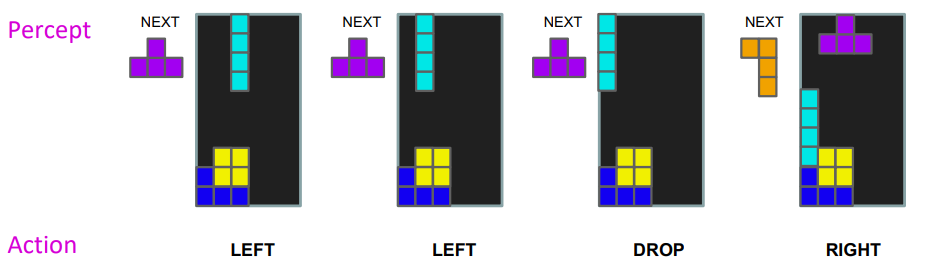
\includegraphics[width=0.7\textwidth]{./pictures/agent_func.png}
        \caption{Représentation fonction agent dans le jeu Tetris}
        \label{fig:agent} 
    \end{figure}
\end{example}

\begin{definition}{Programe Agent}{progagent}
    Un \textbf{programe agent} $l$ est \underline{exécuté} sur une \textbf{machine} $M$ 
    afin d'\underline{implémenter} la fonction agent $f$.
\end{definition}
\begin{remark}\leavevmode
    Les machines dans le monde réel sont \textbf{imparfaites} et \textbf{limitées} en temps et en mémoire.
\end{remark}

\begin{figure}[H]
    \begin{center}
        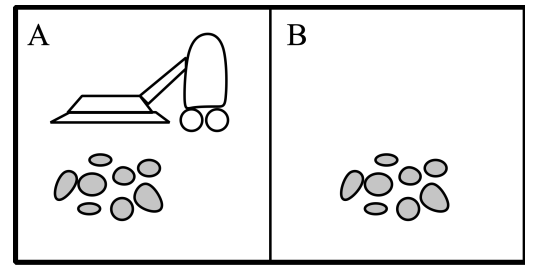
\includegraphics[width=0.25\textwidth]{./pictures/vac_state.png}
    \end{center}
    \caption{Etat de l'environnement de l'aspirateur}\label{fig:vac_state}
\end{figure}

% WARNING: Pas sur que ce soit utile/bonne façon de faire
\begin{example}\leavevmode
    Nous pouvons représenter un aspirateur comme un agent qui perçoit son environnement par des capteurs et agit sur celui-ci par des effecteurs.
    \begin{itemize}
        \item \textbf{Perception}: capteurs qui détectent la saleté et sa localisation dans l'espace
        \item \textbf{Action}: effecteurs qui déplacent l'aspirateur dans l'espace et aspire ou non
    \end{itemize}
    En imaginant la situation en figure \ref{fig:vac_state}, nous pouvons définir la fonction agent de l'aspirateur comme suit:
    \begin{table}[H]
        \caption{Fonction agent de l'aspirateur}\label{tab:agent_func}
        \begin{center}
            \begin{tabular}[c]{|l|l|}
                \hline
                \multicolumn{1}{|c|}{\textbf{Sequence de perception}} & 
                \multicolumn{1}{c|}{\textbf{Action}} \\
                \hline

                [A, Clean] & Right \\
                \hline
                [A, Dirty] & Suck \\
                \hline
                [B, Clean] & Left\\
                \hline
                [B, Dirty] & Suck\\
                \hline
                [A, Clean], [B, Clean] & Left\\
                \hline
                [A, Clean], [B, Dirty] & Suck\\
                \hline
                etc... & etc...\\
                \hline
            \end{tabular}
        \end{center}
    \end{table}
\end{example}

Pour que notre agent soit bien rationnel, il nous faut une manière de \textbf{mesurer} la \textbf{performance}
de celui-ci. Pour cela, nous allons définir une \textbf{fonction de performance} qui va mesurer la qualité des actions de l'agent.

\begin{example}\leavevmode
    On peut lui faire gagner des points ou bien lui en retirer en fonction d'une action
\end{example}
De cette manière, l'agent va savoir quelles actions lui permettent de \textbf{maximiser} son utilité attendue.

Afin de bien déterminer un environnement, les particularité de notre agents, il nous faut 
\textbf{avant toute chose} définir \textbf{\textcolor{red}{PEAS}}

\begin{definition}{PEAS}{peas}
    \begin{itemize}
        \item \textbf{Performance}: mesure de la qualité des actions de l'agent
        \item \textbf{Environnement}: type d'environnement dans lequel l'agent va évoluer
        \item \textbf{Actuateurs}: les effecteurs de l'agent
        \item \textbf{Sensors}: les capteurs de l'agent
    \end{itemize} 
\end{definition}

\begin{figure}[H]
    \begin{center}
        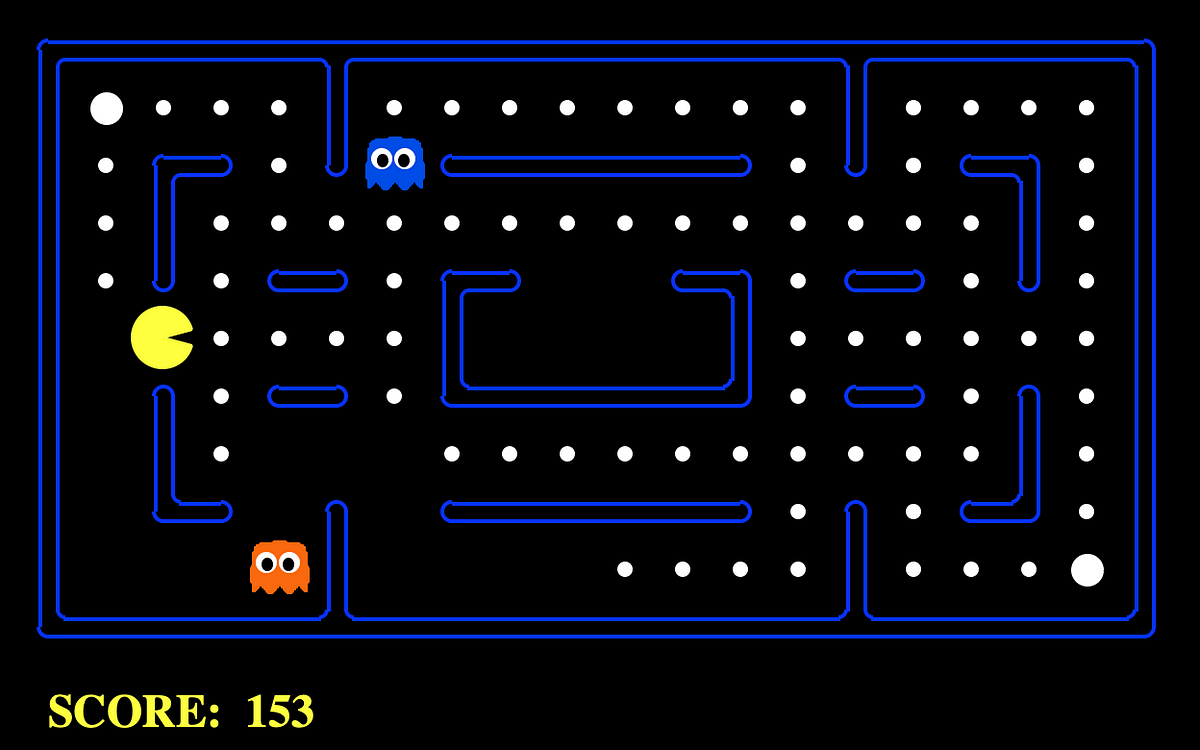
\includegraphics[width=0.25\textwidth]{./pictures/pacman.png}
    \end{center}
    \caption{Environnement Pacman}\label{fig:pacman}
\end{figure}

\begin{example}\leavevmode
    Pour l'environnement Pacman de la figure \ref{fig:pacman}, nous pouvons définir PEAS comme suit:
    \begin{itemize}
        \item \textbf{Performance}: -1/pas, +10/nourriture, +500/partie gagnées, -500/mort, +200/tuer un fantôme effrayé
        \item \textbf{Environnement}: labyrinthe \textbf{dynamique }de pacman
        \item \textbf{Actuateurs}: Haut, Bas, Gauche, Droite
        \item \textbf{Capteurs}: L'état entier visible
    \end{itemize}



\end{example}

\begin{definition}{Types d'environnement}{envtype}
    Il y a plusieur type d'environnement:

    \begin{itemize}
        \item \textbf{Mono-agent}: un seul agent
        \item \textbf{Multi-agent}: plusieurs agents qui maximisent leur \textbf{propre} tâche (coop ou concurentiel)
        \item \textbf{Déterministe}: l'état de l'env est déterminé \textbf{seulement} par les actions de l'agent
        \item \textbf{Stochastique}: l'environnement est non déterministe
        \item \textbf{Épisodique}: les actions de l'agent n'affectent pas les actions futures
        \item \textbf{Séquentiel}: les actions de l'agent affectent les actions futures
        \item \textbf{Dynamique}: l'environnement peut changer pendant que l'agent réfléchit
        \item \textbf{Statique}: l'environnement ne change pas pendant que l'agent réfléchit
        \item \textbf{Complètement observable}: les capteurs de l'agent perçoivent l'état complet de l'environnement
        \item \textbf{Partiellement observable}: les capteurs de l'agent perçoivent une partie de l'état de l'environnement
        \item \textbf{Discret}: un nombre fini d'états
        \item \textbf{Continu}: un nombre infini d'états
        \item \textbf{Connu}: l'agent connait les lois de l'environnement
    \end{itemize}
\end{definition}

Il existe plusieurs types d'agents qui répondent à des environnements plus complexes:
\begin{itemize}
    \item \textbf{Agent réflexe simple}: l'agent choisit son action en fonction de la \textbf{dernière} perception
    \item \textbf{Agent réflexe basé sur un modèle}: l'agent choisit son action en fonction de la \textbf{dernière} perception et d'un \textbf{état interne}(dépend de l'\textbf{historique} des perceptions) 
    % \item \textbf{Agent réflexe avec état}: l'agent choisit son action en fonction de la \textbf{dernière} perception et de l'\textbf{historique} des perceptions
    \item \textbf{Agent fondés sur des buts}: l'agent choisit son action en fonction de la dernière perception 
        ainsi que des infos relatives à l'objectif
    \item \textbf{Agent fondés sur l'utilité}: l'agent choisit son action en fonction de 
        sa satisfaction par rapport à l'état résultant
\end{itemize}
